\section{Characterization of the light sheet}
\label{sec:LightSheet}

As a first step we has to characterize the light sheet used in the following section. This is done by analyzing the intensity profile 
of the beam after the collimators. As the used solution is homogeneous, an we are at relatively low intensity, we can 
assume that the scattering light collected with the second collimator is proportional to the intensity in those points.

The analysis follows three steps. First all 100 images are averaged. A Savgol filter is applied to the image.
The beam is a Gaussian beam as can be seen in \cref{fig:subfigureBeamshape} having the form
\begin{equation}
    E(r, z)=E_0 \frac{w_0}{w(z)} \cdot \mathrm{e}^{-\left(\frac{r}{w(z)}\right)^2} \cdot \mathrm{e}^{-i k \frac{r^2}{2 R(z)}} \cdot \mathrm{e}^{-i(k z-\zeta(z))}.
\end{equation}
For the characterization, the transversal profile is important, which is represented in the first exponential term. The $w(z)$ represents the beam radius. 
In general the beam radius is given by 
\begin{equation}
    w(z) = w_0 \sqrt{1+\left(\frac{z}{z_r}\right)^2}
\end{equation} 
with $z_r$ being the rayleigh length. When taking $z=0$ we extract $w_0$ taking a 1D Gaussian fit.

The Rayleigh length can be extracted by observing the divergence 
\begin{equation}
    \theta_{\mathrm{div}} = \lim_{z \to \infty} \arctan\left(\frac{w(z)}{z}\right) = \frac{w_0}{z_R}
\end{equation}
of the beam. 

\begin{figure}[ht]
    \centering
    \begin{subfigure}{0.95\linewidth}
      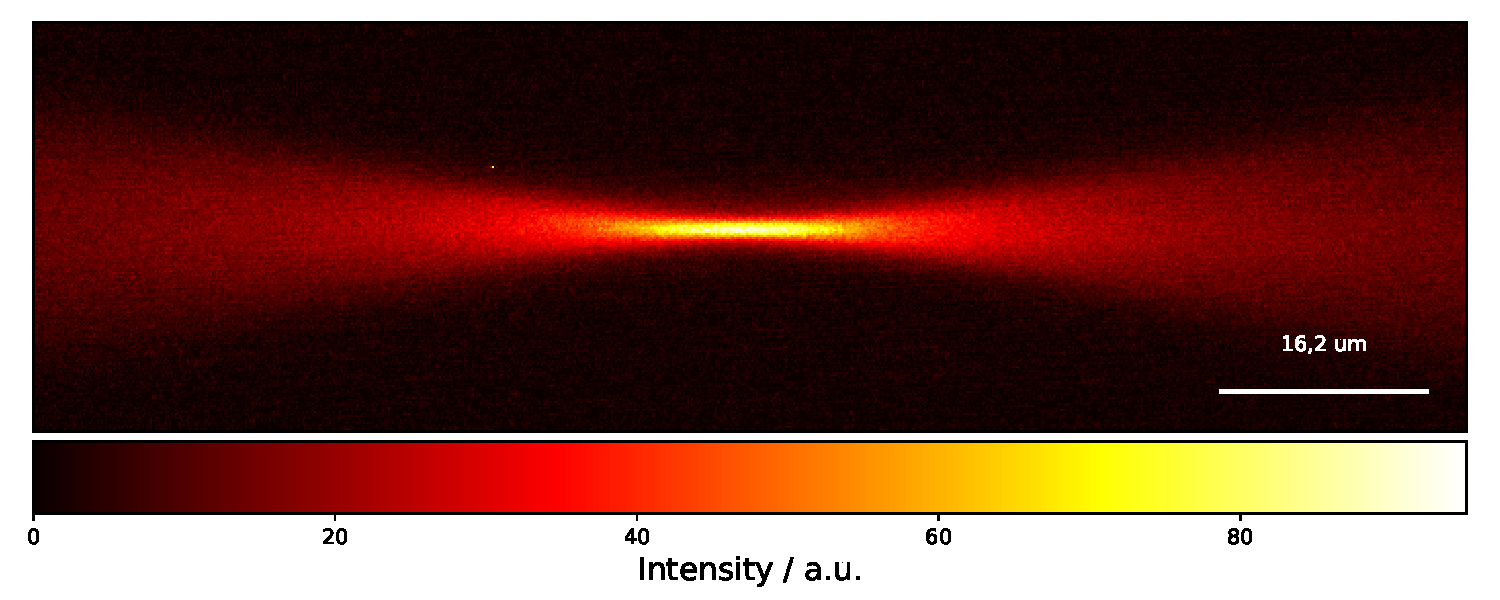
\includegraphics[width=\linewidth]{data/lightsheetCharacterization/NoPinhole/LSC_nopinhole_40ms_100_1/LSNiPinhole.pdf}
      \caption{No pinhole}
      \label{fig:subfig1}
    \end{subfigure}

    \begin{subfigure}{0.95\linewidth}
      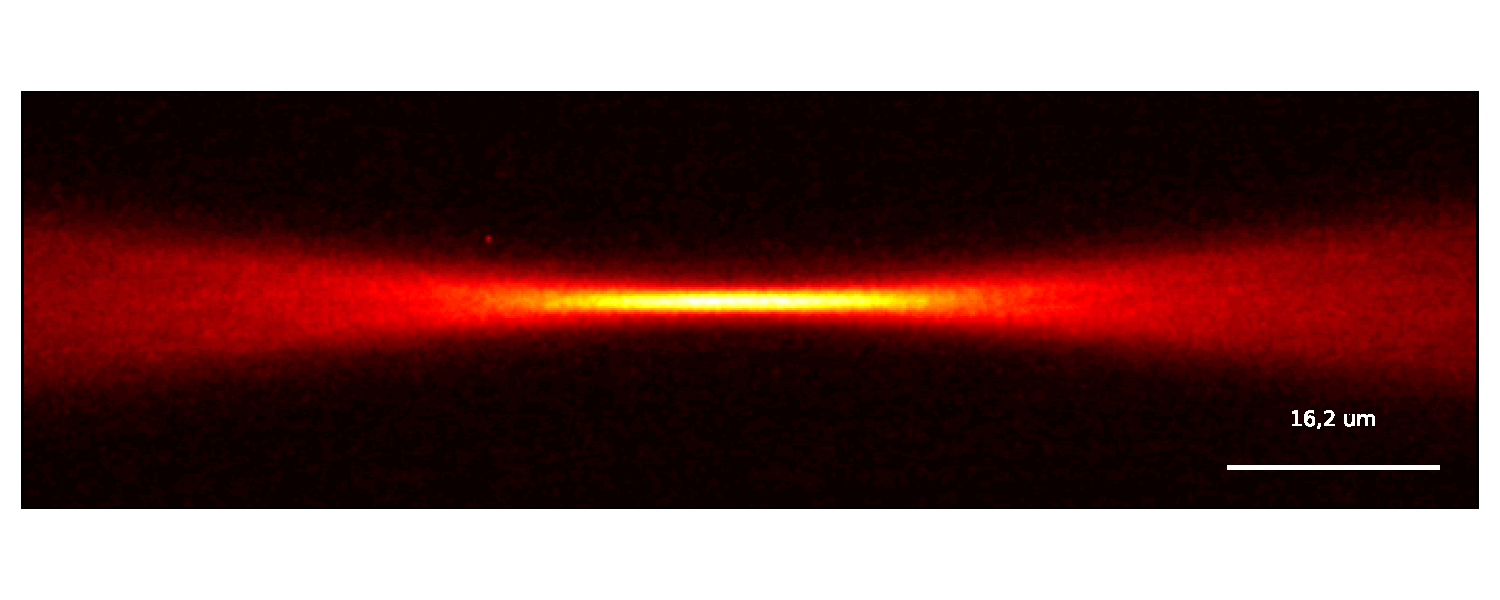
\includegraphics[width=\linewidth]{data/lightsheetCharacterization/HalfClosedPinhole/LSC_halfclosedpinhole_40ms_100_1/LSHalfPinhole.pdf}
      \caption{Half closed pinhole}
      \label{fig:subfig2}
    \end{subfigure}

    \begin{subfigure}{0.95\linewidth}
      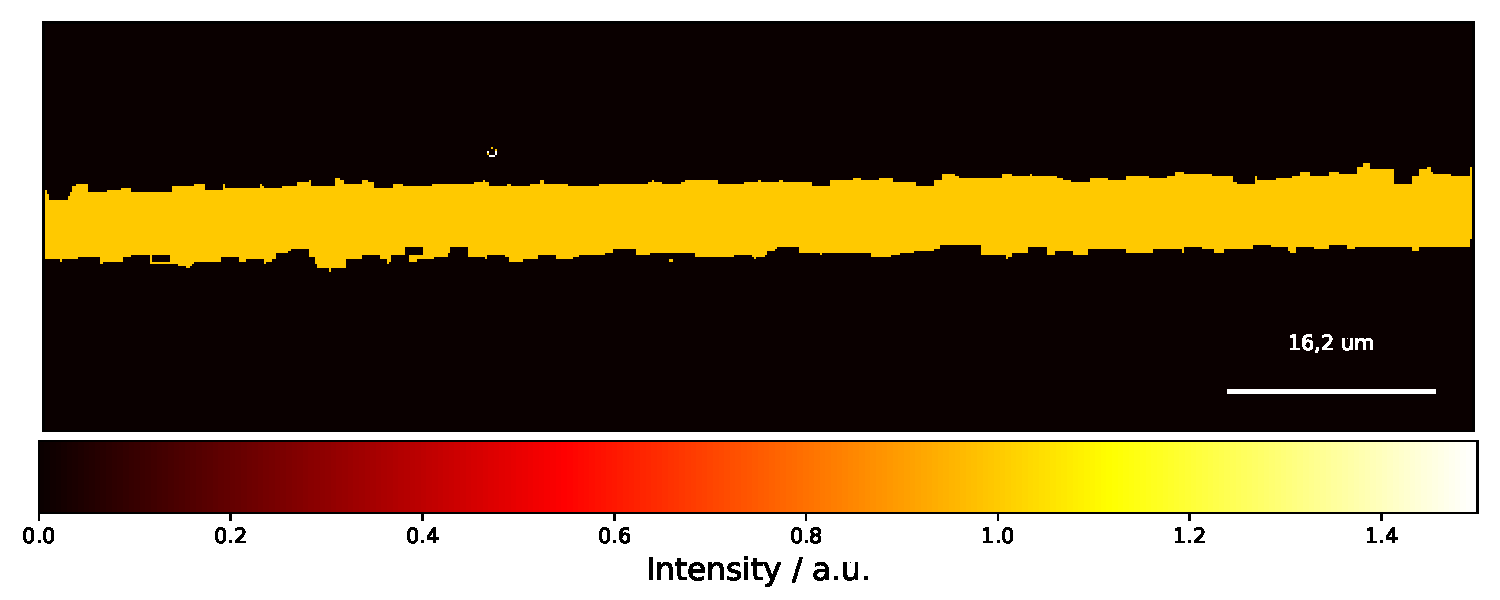
\includegraphics[width=\linewidth]{data/lightsheetCharacterization/ClosedPinhole/LSC_closedpinhole_40ms_2_7A_1/LSPinhole.pdf}
      \caption{Closed pinhole}
      \label{fig:subfig3}
    \end{subfigure}

    \caption{Images of the scattered light from a beam focused by a collimator. }
    \label{fig:subfigureBeamshape}
\end{figure}

The beam width from the fit for the beam without pinhole is $w_{\mathrm{0}}^{\mathrm{no-ph}} = \SI{1.03\pm0.02}{\micro\meter}$, whereas the half closed pinhole narrows down the beam waist to $w_{\mathrm{0}}^{\mathrm{hc-ph}} = \SI{0.96\pm0.02}{\micro\meter}$. The 
divergence angels are $\theta_{\mathrm{div}}^{\mathrm{no-ph}} = \SI{0.17\pm0.01}{rad}$ and $\theta_{\mathrm{div}}^{\mathrm{hc-ph}} = \SI{0.10\pm0.01}{rad}$ and therefore the $z_{\mathrm{R}}^{\mathrm{no-ph}} = \SI{6.0\pm0.6}{\micro\meter}$ and
$z_{\mathrm{R}}^{\mathrm{hc-ph}} = \SI{9.6\pm0.9}{\micro\meter}$.

The fully closed pinhole does not allow a suitable analysis as the intensity is to low. Nevertheless, it should have a beam waste below the half closed pinhole. 
The tendency for the beam waste to shrink when the pinhole is half closed is to be expected as we cut out the outer parts of the beam.
The change in the Rayleigh length is a mystery for us that requires further consideration.